\section*{Domácí úloha 1}

\subsection*{Příklad č.~1}

Dokažte nebo vyvraťte protipříkladem následující tvrzení. Pro všechny množiny $X,Y,Z \subseteq U$ platí (doplňky množin uvažujeme vůči množině $U$):

\begin{equation}
\overline{X \cap Y} = \overline{X} \cup \overline{Y} \label{eq:1.1}
\end{equation}

Tvrzení \eqref{eq:1.1} je pravdivé.

\textbf{Důkaz:}
\begin{eqnarray*}
x \in \overline{X \cap Y} &\Rightarrow&
x \in U \setminus (X \cap Y) \Rightarrow \\ &\Rightarrow&
x \in U \wedge x \not\in (X \cap Y) \Rightarrow \\ &\Rightarrow&
x \in U \wedge (x \not\in X \vee x \not\in Y) \Rightarrow \\ &\Rightarrow&
(x \in U \wedge x \not\in X) \vee (x \in U \wedge x \not\in Y) \Rightarrow \\ &\Rightarrow&
(x \in U \setminus X) \vee (x \in U \setminus Y) \Rightarrow \\ &\Rightarrow&
x \in \overline{X} \vee x \in \overline{Y} \Rightarrow \\ &\Rightarrow&
x \in \overline{X} \cup \overline{Y}
\end{eqnarray*}
\begin{eqnarray*}
x \in \overline{X} \cup \overline{Y} &\Rightarrow&
(x \in U \setminus X) \vee (x \in U \setminus Y) \Rightarrow \\ &\Rightarrow&
(x \in U \wedge x \not\in X) \vee (x \in U \wedge x \not\in Y) \Rightarrow \\ &\Rightarrow&
x \in U \wedge (x \not\in X \vee x \not\in Y) \Rightarrow \\ &\Rightarrow&
x \in U \wedge x \not\in (X \cap Y) \Rightarrow \\ &\Rightarrow&
x \in U \setminus (X \cap Y) \Rightarrow \\ &\Rightarrow&
x \in \overline{X \cap Y}
\end{eqnarray*}

\noindent\rule{\textwidth}{1pt}

\begin{equation}
Y \setminus X = X \setminus Y \label{eq:1.2}
\end{equation}

Tvrzení \eqref{eq:1.2} není pravdivé.

\textbf{Důkaz:}
\begin{eqnarray*}
X \setminus Y &\Rightarrow& x \in X \wedge x \not\in Y \\
Y \setminus X &\Rightarrow& x \in Y \wedge x \not\in X
\end{eqnarray*}
\begin{eqnarray*}
X &=& \lbrace 1, 2, 3, 4 \rbrace \\
Y &=& \lbrace 3, 4, 5, 6 \rbrace \\
Y \setminus X &\neq& X \setminus Y \\
\lbrace 5, 6\rbrace &\neq& \lbrace 1, 2 \rbrace
\end{eqnarray*}

%\noindent\rule{\textwidth}{1pt}
\newpage

\begin{equation}
\overline{X \cup Y} \supseteq X \label{eq:1.3}
\end{equation}

Tvrzení \eqref{eq:1.3} není pravdivé, protože $\overline{X \cup Y}$ je množina všeho, co nenáleží do $X$ ani do $Y$.

\textbf{Důkaz:}
\begin{eqnarray*}
X &=& \lbrace 1, 2 \rbrace \\
Y &=& \lbrace 2, 3 \rbrace
\end{eqnarray*}
\begin{eqnarray*}
X \cup Y &=& \lbrace 1, 2, 3 \rbrace \\
\overline{X \cup Y} &=& U \setminus \lbrace 1, 2, 3 \rbrace \\
U \setminus \lbrace 1, 2, 3 \rbrace &\not\supseteq& \lbrace 1,2 \rbrace
\end{eqnarray*}

\noindent\rule{\textwidth}{1pt}

\begin{equation}
(X \cup Y) \cap (Y \setminus X) = Y \label{eq:1.4}
\end{equation}

Tvrzení \eqref{eq:1.4} není pravdivé.

\textbf{Důkaz:}
\begin{eqnarray*}
X &=& \lbrace 1, 2 \rbrace \\
Y &=& \lbrace 2, 3 \rbrace
\end{eqnarray*}
\begin{eqnarray*}
(X \cup Y) \cap (Y \setminus X) &=&
(\lbrace 1, 2 \rbrace \cup \lbrace 2, 3 \rbrace) \cap (\lbrace 2, 3 \rbrace \setminus \lbrace 1, 2 \rbrace) = \\ &=&
\lbrace 1, 2, 3 \rbrace \cap \lbrace 3 \rbrace = \\ &=&
\lbrace 3 \rbrace \\
(X \cup Y) \cap (Y \setminus X) &\neq& Y
\end{eqnarray*}

\noindent\rule{\textwidth}{1pt}

\begin{equation}
X \setminus (Y \cap Z) = (X \setminus Y) \cup Z \label{eq:1.5}
\end{equation}

Tvrzení \eqref{eq:1.5} není pravdivé.

\textbf{Důkaz:}
\begin{eqnarray*}
X &=& \lbrace a, b, c, d \rbrace \\
Y &=& \lbrace a, b, 1, 2 \rbrace \\
Z &=& \lbrace a, c, 1, 3 \rbrace
\end{eqnarray*}
\begin{eqnarray*}
X \setminus (Y \cap Z) &=&
\lbrace a, b, c, d \rbrace \setminus (\lbrace a, b, 1, 2 \rbrace \cap \lbrace a, c, 1, 3 \rbrace)  = \\ &=&
\lbrace a, b, c, d \rbrace \setminus \lbrace a, 1 \rbrace = \\ &=&
\lbrace b, c, d \rbrace \\
(X \setminus Y) \cup Z &=&
(\lbrace a, b, c, d \rbrace \setminus \lbrace a, b, 1, 2 \rbrace) \cup \lbrace a, c, 1, 3 \rbrace \\ &=&
\lbrace c, d \rbrace \cup \lbrace a, c, 1, 3 \rbrace = \\ &=&
\lbrace a, c, d, 1, 3 \rbrace \\
\lbrace b, c, d \rbrace &\neq& \lbrace a, c, d, 1, 3 \rbrace \\
X \setminus (Y \cap Z) &\neq& (X \setminus Y) \cup Z
\end{eqnarray*}

\newpage

\subsection*{Příklad č.~2}

Na množině $X = \lbrace 1, 2, 3, 4, 5, 6, 7, 8 \rbrace$ je dána relace $R = \lbrace (x,y)\mid x, y \in X, 3x \text{ dělí } 4y\rbrace$. Zapište relaci $R$ výčtem prvků. Určete její definiční obor a obor hodnot. Nalezněte
relaci $R^{-1}$.

\begin{center}
\setlength{\arrayrulewidth}{1.5pt}
\renewcommand{\arraystretch}{1.5}
\Large
\begin{tabular}{|c|c|c|c|c|c|c|c|c|c|}
\hline
~ & x                & 1              & 2              & 3               & 4               & 5               & 6              & 7               & 8               \\
\hline
y & \diagbox{3x}{4y} & 4              & 8              & 12              & 16              & 20              & 24             & 28              & 32              \\
\hline
1 & 3                & $\frac{4}{3}$  & $\frac{8}{3}$  & \enlCell{4}     & $\frac{3}{16}$  & $\frac{20}{3}$  & \enlCell{8}    & $\frac{28}{3}$  & $\frac{32}{3}$  \\
\hline
2 & 6                & $\frac{2}{3}$  & $\frac{4}{3}$  & \enlCell{2}     & $\frac{3}{8}$   & $\frac{10}{3}$  & \enlCell{4}    & $\frac{14}{3}$  & $\frac{16}{3}$  \\
\hline
3 & 9                & $\frac{4}{9}$  & $\frac{8}{9}$  & $\frac{4}{3}$   & $\frac{9}{16}$  & $\frac{20}{9}$  & $\frac{24}{9}$ & $\frac{28}{9}$  & $\frac{32}{9}$  \\
\hline
4 & 12               & $\frac{1}{3}$  & $\frac{12}{9}$ & \enlCell{1}     & $\frac{3}{4}$   & $\frac{5}{3}$   & \enlCell{2}    & $\frac{7}{3}$   & $\frac{8}{3}$   \\
\hline
5 & 15               & $\frac{4}{15}$ & $\frac{5}{3}$  & $\frac{4}{5}$   & $\frac{16}{15}$ & $\frac{5}{4}$   & $\frac{8}{5}$  & $\frac{28}{15}$ & $\frac{32}{15}$ \\
\hline
6 & 18               & $\frac{2}{9}$  & $\frac{4}{9}$  & $\frac{2}{3}$   & $\frac{8}{9}$   & $\frac{10}{9}$  & $\frac{4}{3}$  & $\frac{14}{9}$  & $\frac{16}{9}$  \\
\hline
7 & 21               & $\frac{4}{21}$ & $\frac{8}{21}$ & $\frac{12}{21}$ & $\frac{16}{21}$ & $\frac{20}{21}$ & $\frac{8}{7}$  & $\frac{4}{3}$   & $\frac{32}{21}$ \\
\hline
8 & 24               & $\frac{1}{6}$  & $\frac{1}{3}$  & $\frac{1}{2}$   & $\frac{4}{6}$   & $\frac{5}{6}$   & \enlCell{1}    & $\frac{14}{12}$ & $\frac{4}{3}$   \\
\hline
\end{tabular}
\end{center}

\begin{eqnarray*}
R &=& \lbrace (1, 3), (1, 6), (2, 3), (2, 6), (4, 3), (4, 6), (8,6) \rbrace \\
Dom~R &=& \lbrace 1, 2, 4, 8 \rbrace \\
Im~R &=& \lbrace 3, 6 \rbrace \\
R^{-1} &=& \lbrace (3, 1), (6, 1), (3, 2), (6, 2), (3, 4), (6, 4), (6, 8) \rbrace
\end{eqnarray*}

\newpage

\subsection*{Příklad č.~3}

Uvažujte množinu $\tau_{n}$ všech topologií na množině o $n = 2$ prvcích s uspořádáním
inkluzí. Nakreslete její Hasseův diagram a rozhodněte, zda je $(\tau_{2}, \subseteq)$ svazově uspořádaná.

\begin{eqnarray*}
X &=& \lbrace 1, 2 \rbrace \\
2^{X} &=& \lbrace \emptyset, \lbrace 1 \rbrace, \lbrace 2 \rbrace, \lbrace 1, 2 \rbrace \rbrace \\
\tau_{n} &=& \lbrace
\lbrace \emptyset, \lbrace 1, 2 \rbrace \rbrace,
\lbrace \emptyset, \lbrace 1 \rbrace, \lbrace 2 \rbrace, \lbrace 1, 2 \rbrace \rbrace,
\lbrace \emptyset, \lbrace 1 \rbrace, \lbrace 1, 2 \rbrace \rbrace,
\lbrace \emptyset, \lbrace 2 \rbrace, \lbrace 1, 2 \rbrace \rbrace
\rbrace
\end{eqnarray*}
\minipage{0.50\textwidth}
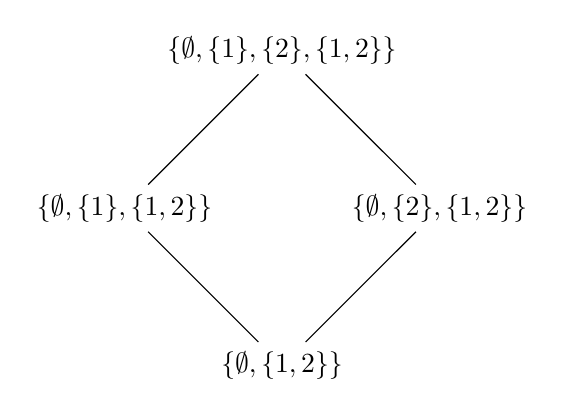
\begin{tikzpicture}
  \node (one) at (0,2) {$\lbrace \emptyset, \lbrace 1 \rbrace, \lbrace 2 \rbrace, \lbrace 1, 2 \rbrace \rbrace$};
  \node (a) at (-2,0) {$\lbrace \emptyset, \lbrace 1 \rbrace, \lbrace 1, 2 \rbrace \rbrace$};
  \node (b) at (2,0) {$\lbrace \emptyset, \lbrace 2 \rbrace, \lbrace 1, 2 \rbrace \rbrace$};
  \node (zero) at (0,-2) {$\lbrace \emptyset, \lbrace 1, 2 \rbrace \rbrace$};
  \draw (zero) -- (a) -- (one) -- (b) -- (zero);
\end{tikzpicture}
\endminipage
\minipage{0.50\textwidth}
\begin{eqnarray*}
\inf \tau_{2} &=& \lbrace \emptyset, \lbrace 1, 2 \rbrace \rbrace \\
\sup \tau_{2} &=& \lbrace \emptyset, \lbrace 1 \rbrace, \lbrace 2 \rbrace, \lbrace 1, 2 \rbrace \rbrace
\end{eqnarray*}
Množina $(\tau_{2}, \subseteq)$ je svazově uspořádaná, protože má v $\tau_{2}$ infimum i supremum.
\endminipage

\subsection*{Příklad č.~4}

\setcounter{equation}{0}

Dokažte nebo vyvraťte protipříkladem pro libovolné dvě relace $R_{1}, R_{2}$ na množině $X$:

\begin{equation}
\rho (R_{1} \cup R_{2}) = \rho (R_{1}) \cup \rho (R_{2})\label{eq:4.1}
\end{equation}

Tvrzení \eqref{eq:4.1} je pravdivé.

\textbf{Důkaz:}
\begin{eqnarray*}
\rho (R_{1} \cup R_{2}) &=&
R_{1} \cup R_{2} \cup \Delta X = \\ &=&
(R_{1} \cup \Delta X) \cup (R_{2} \cup \Delta X) = \\ &=&
\rho (R_{1}) \cup \rho (R_{2})
\end{eqnarray*}

\noindent\rule{\textwidth}{1pt}

\begin{equation}
\sigma (R_{1} \cap R_{2}) = \sigma (R_{1}) \cap \sigma (R_{2})\label{eq:4.2}
\end{equation}

Tvrzení \eqref{eq:4.2} není pravdivé.

\textbf{Důkaz:}
\begin{eqnarray*}
R_{1} &=& \lbrace (1, 2) \rbrace \\
R_{2} &=& \lbrace (2, 1) \rbrace \\
R_{1} \cap R_{2} &=& \emptyset \\
\sigma(R_{1}) =
\lbrace (1, 2) \cup (2, 1) \rbrace &=&
\lbrace (1, 2), (2, 1) \rbrace \\
\sigma(R_{2}) &=&
\lbrace (2, 1) \cup (1, 2) \rbrace = \\ &=&
\lbrace (1, 2), (2, 1) \rbrace \\
\emptyset &\neq& \lbrace (1, 2), (2, 1) \rbrace \\
\sigma (R_{1} \cap R_{2}) &\neq& \sigma (R_{1}) \cap \sigma (R_{2})
\end{eqnarray*}

%\noindent\rule{\textwidth}{1pt}
\newpage

\begin{equation}
\tau (R_{1} \cap R_{2}) = \tau (R_{1}) \cap \tau (R_{2})\label{eq:4.3}
\end{equation}

Tvrzení \eqref{eq:4.3} není pravdivé.

\textbf{Důkaz:}
\begin{eqnarray*}
R_{1} &=& \lbrace (1, 2), (2, 3), (3, 1) \rbrace \\
R_{2} &=& \lbrace (1, 2), (2, 5), (5, 1) \rbrace \\
\tau(R_{1}) &=& \lbrace (1, 2), (2, 3), (3, 1), (1, 3), (2, 1), (3, 2) \rbrace \\
\tau(R_{2}) &=& \lbrace (1, 2), (2, 5), (5, 1), (1, 5), (2, 1), (5, 2) \rbrace \\
\tau (R_{1}) \cap \tau (R_{2}) &=& \lbrace (1, 2), (2, 1) \rbrace \\
R_{1} \cap R_{2} &=& \lbrace (1,2) \rbrace \\
\tau(R_{1} \cap R_{2}) &=& \lbrace (1,2) \rbrace \\
\tau (R_{1} \cap R_{2}) &\neq& \tau (R_{1}) \cap \tau (R_{2})
\end{eqnarray*}

\noindent\rule{\textwidth}{1pt}

\begin{equation}
\tau (R_{1} \cup R_{2}) = \tau (R_{1}) \cup \tau (R_{2})\label{eq:4.4}
\end{equation}

Tvrzení \eqref{eq:4.4} není pravdivé.

\textbf{Důkaz:}
\begin{eqnarray*}
R_{1} &=& \lbrace (1, 2), (2, 1) \rbrace \\
R_{2} &=& \lbrace (2, 3), (3, 2) \rbrace \\
\tau(R_{1}) &=& \lbrace (1, 1), (1, 2), (2, 1), (2, 2) \rbrace \\
\tau(R_{2}) &=& \lbrace (2, 2), (2, 3), (3, 2), (3, 3) \rbrace
\end{eqnarray*}
\begin{eqnarray*}
R_{1} \cup R_{2} &=& \lbrace (1, 2), (2, 1), (2, 3), (3, 2) \rbrace \\
\tau (R_{1} \cup R_{2}) &=& \lbrace (1, 1), (1, 2), (2, 1), (2, 2), (2, 3), (3, 2), (3, 3), (1, 3), (3, 1) \rbrace \\
\tau (R_{1}) \cup \tau (R_{2}) &=& \lbrace (1, 1), (1,2), (2, 1), (2, 2), (2, 3), (3, 2), (3, 3) \rbrace \\
\tau (R_{1} \cup R_{2}) &\neq& \tau (R_{1}) \cup \tau (R_{2})
\end{eqnarray*}

%\noindent\rule{\textwidth}{1pt}
\newpage

\begin{equation}
\sigma(\rho(R_{1})) = \rho(\sigma(R_{1}))\label{eq:4.5}
\end{equation}

Tvrzení \eqref{eq:4.5} je pravdivé.

\textbf{Důkaz:}
\begin{eqnarray*}
\sigma(\rho(R_{1})) &=&
\sigma(R_{1} \cup \Delta X) = \\ &=&
(R_{1} \cup \Delta X) \cup (R_{1} \cup \Delta X)^{-1} = \\ &=&
(R_{1} \cup \Delta X) \cup (R_{1}^{-1} \cup \Delta X^{-1}) = \\ &=&
(R_{1} \cup R_{1}^{-1}) \cup (\Delta X \cup \Delta X^{-1}) = \\ &=&
\sigma(R_{1}) \cup (\Delta X \cup \Delta X^{-1}) = \\ &=&
\rho(\sigma(R_{1}))
\end{eqnarray*}

\noindent\rule{\textwidth}{1pt}

\begin{equation}
\sigma(\tau(R_{1})) = \tau(\sigma(R_{1}))\label{eq:4.6}
\end{equation}

Tvrzení \eqref{eq:4.6} není pravdivé.

\textbf{Důkaz:}
\begin{eqnarray*}
R_{1} &=& \lbrace (1, 2), (2, 3) \rbrace \\
\tau(R_{1}) &=& \lbrace (1, 2), (2, 3), (1, 3) \rbrace \\
\sigma(\tau(R_{1})) &=& \lbrace (1, 2), (2, 3), (1, 3), (2, 1), (3, 2), (3, 1) \rbrace \\
\sigma(R_{1}) &=& \lbrace (1, 1), (2, 2), (3, 3), (2, 1), (2, 3), (1, 2), (3, 2), (1, 3), (3, 1) \rbrace \\
\tau(\sigma(R_{1})) &=& \lbrace (1, 1), (2, 2), (3, 3), (2, 1), (2, 3), (1, 2), (3, 2), (1, 3), (3, 1) \rbrace \\
\sigma(\tau(R_{1})) &\neq& \tau(\sigma(R_{1}))
\end{eqnarray*}

\noindent\rule{\textwidth}{1pt}

\begin{equation}
\rho(\tau(R_{1})) = \tau(\rho(R_{1}))\label{eq:4.7}
\end{equation}

Tvrzení \eqref{eq:4.7} je pravdivé.

\textbf{Důkaz:}
\begin{eqnarray*}
R_{1} &=& \lbrace (1, 2), (2, 3) \rbrace \\
\tau(R_{1}) &=& \lbrace (1, 2), (2, 3), (1, 3) \rbrace \\
\rho(\tau(R_{1})) &=& \lbrace (1, 1), (2, 2), (3, 3), (1, 2), (2, 3), (1, 3) \rbrace \\
\rho(R_{1}) &=& \lbrace (1, 1), (1, 2), (2, 3), (2, 2), (3, 3) \rbrace \\
\tau(\rho(R_{1})) &=& \lbrace (1, 1), (2, 2), (3, 3), (2, 3), (1, 2), (1, 3) \rbrace \\
\rho(\tau(R_{1})) &=& \tau(\rho(R_{1})) \\
\rho(R_{1} \circ R_{2}) &=&
(R_{1} \circ R_{2}) \cup (\Delta X \circ \Delta X) = \\ &=&
(R_{1} \cup \Delta X) \circ (R_{2} \cup \Delta X) = \\ &=&
\tau(R_{1} \cup \Delta X) = \\ &=&
\tau(\rho(R_{1}))
\end{eqnarray*}

\newpage

\subsection*{Příklad č.~5}

Položme $X = \lbrace 0, 1, 2, 3, 4, 5 \rbrace$ a $Y
= \lbrace 0 , 1, 2 \rbrace$. Dále klademe $x_{1} \oplus x_{2} = (x_{1} + x_{2}) \mod 6$, $x_{1} \odot x_{2} = (x_{1} \cdot x_{2}) \mod 6$, $y_{1} \boxplus y_{2} = (y_{1} + y_{2}) \mod 3$, $y_{1} \boxdot y_{2} = (y_{1} \cdot y_{2}) \mod 3$ pro všechna $x_{1}, x_{2} \in X$ a $y_{1}, y_{2} \in Y$. Dokažte, že $f: X \rightarrow Y$, kde $f(x) = x \mod 3$ je morfismus algeber $(X, \oplus, \odot)$ a $(Y, \boxplus, \boxdot)$. Nalezněte Ker $f$ a sestrojte faktorovou algebru $X$/Ker $f$. Faktorizujte zobrazení $f$ přes faktorovou algebru.

\begin{eqnarray*}
X &=& \lbrace 0, 1, 2, 3, 4, 5 \rbrace \\
Y &=& \lbrace 0 , 1, 2 \rbrace \\
x_{1} \oplus x_{2} &:=& (x_{1} + x_{2}) \mod 6 \\
x_{1} \odot x_{2} &:=& (x_{1} \cdot x_{2}) \mod 6 \\
y_{1} \boxplus y_{2} &:=& (y_{1} + y_{2}) \mod 3 \\
y_{1} \boxdot y_{2} &:=& (y_{1} \cdot y_{2}) \mod 3
\end{eqnarray*}

\begin{eqnarray*}
f(x_{1} \oplus x_{2}) &=& f(x_{1}) \boxplus f(x_{2}) \\
x_{1} + x_{2} &=& 6k + r; k, r \in \mathbb{Z}; 0 \leq r < 6 \\
x_{1} \oplus x_{2} &=& r = 3v + s; v,s \in \mathbb{Z}; 0 \leq s < 3 \\
x_{1} &=& 3m + t; m, t \in \mathbb{Z}; 0 \leq t < 3 \\
x_{2} &=& 3p + u; p, u \in \mathbb{Z}; 0 \leq u < 3 \\
f(x_{1}) &=& t; f(x_{2}) = u \\
t + u &=& 3q + v, \text{kde}~ q,v \in \mathbb{Z}; 0 \leq u < 3 \\
f(x_{1}) \boxplus f(x_{2}) &=& (t + u) \mod 3 = v \\
x_{1} + x_{2} &=& 6k + r = 6k + 3v + s = 3 \cdot (2k + v) + s \Rightarrow (x_{1} + x_{2}) \mod 3 = s \\
x_{1} + x_{2} &=&  3m + 3p + 3q +v = 3 \cdot (m + p + q) + v \Rightarrow (x_{1} + x_{2}) \mod 3 = v \\
f(x_{1} \oplus x_{2}) &=& s = f(x_{1}) \boxplus f(x_{2}) \\
\end{eqnarray*}

\begin{eqnarray*}
f(x_{1} \odot x_{2}) &=& f(x_{1}) \boxdot f(x_{2}) \\
x_{1} \cdot x_{2} &=& 6k + r; k, r \in \mathbb{Z}; 0 \leq r < 6 \\
x_{1} \odot x_{2} &=& r = 3m + s; m, s \in \mathbb{Z}; 0 \leq s < 3 \\
x_{1} &=& 3n + t; n, t \in \mathbb{Z}, 0 \leq t < 3 \\
x_{2} &=& 3p + u; p, u \in \mathbb{Z}, 0 \leq u < 3 \\
f(x_{1}) &=& t; f(x_{2}) = u \\
t \cdot u &=& 3q + v; q, v \in \mathbb{Z}, 0 \leq v < 3 \\
f(x_{1}) \boxdot f(x_{2}) &=& (t \cdot u) \mod 3 = v \\
x_{1} \cdot x_{2} &=& 6k+r = 6k+3m+s = 3(2k + m)+s \Rightarrow (x_{1} \cdot x_{2}) \mod 3 = s \\
x_{1} \cdot x_{2} &=& 3n + 3p + 3q + v = 3 (n + p + q) + v \Rightarrow (x_{1} \cdot x_{2}) \mod 3 = v \\
f(x_{1} \odot x_{2}) &=& s = f(x_{1}) \boxdot f(x_{2})
\end{eqnarray*}

\begin{eqnarray*}
\ker f &=& f^{-1} \circ f = \\
&=& \lbrace (x;y) \mid x,y \in X, f(x) = f(y) \rbrace \\
\varrho &=& X / \ker f = \\
&=&  \lbrace \lbrace 0, 3 \rbrace, \lbrace 1, 4 \rbrace, \lbrace 2, 5 \rbrace \rbrace \\
\left[x\right] \bigoplus \left[y\right] &:=& \left[x \oplus y\right] \\
\left[x\right] \bigodot \left[y\right] &:=& \left[x \odot y\right] \\
\end{eqnarray*}

\begin{center}
\begin{tabular}{|c|c|c|c|}
\hline 
$\bigodot$             & $\lbrace 0, 3 \rbrace$ & $\lbrace 1,4 \rbrace$ & $\lbrace 2,5 \rbrace$ \\ 
\hline 
$\lbrace 0, 3 \rbrace$ & $\lbrace 0, 3 \rbrace$ & $\lbrace 0, 3 \rbrace$ & $\lbrace 0, 3 \rbrace$ \\ 
\hline 
$\lbrace 1, 4 \rbrace$ & $\lbrace 0, 3 \rbrace$ & $\lbrace 1, 4 \rbrace$ & $\lbrace 2, 5 \rbrace$ \\ 
\hline 
$\lbrace 2, 5 \rbrace$ & $\lbrace 0, 3 \rbrace$ & $\lbrace 2, 5 \rbrace$ & $\lbrace 1, 4 \rbrace$ \\ 
\hline 
\end{tabular}
\begin{tabular}{|c|c|c|c|}
\hline 
$\bigoplus$            & $\lbrace 0, 3 \rbrace$ & $\lbrace 1,4 \rbrace$ & $\lbrace 2,5 \rbrace$ \\ 
\hline 
$\lbrace 0, 3 \rbrace$ & $\lbrace 0, 3 \rbrace$ & $\lbrace 1, 4 \rbrace$ & $\lbrace 2, 5 \rbrace$ \\ 
\hline 
$\lbrace 1, 4 \rbrace$ & $\lbrace 1, 4 \rbrace$ & $\lbrace 2, 5 \rbrace$ & $\lbrace 0, 3 \rbrace$ \\ 
\hline 
$\lbrace 2, 5 \rbrace$ & $\lbrace 2, 5 \rbrace$ & $\lbrace 0, 3 \rbrace$ & $\lbrace 1, 4 \rbrace$ \\ 
\hline 
\end{tabular}
\end{center}

\begin{figure}
\centering
\begin{tikzpicture}
  \matrix (m) [matrix of math nodes, row sep=1em, column sep=4em]
    {
    0 & \lbrace 0, 3 \rbrace & 0 \\
    1 & \lbrace 1, 4 \rbrace & 1 \\
    2 & \lbrace 2, 5 \rbrace & 2 \\
    3 \\
    4 \\
    5 \\
    };
    {
    [start chain]
    \chainin (m-1-1);
    \chainin (m-1-2) [join={node[above,labeled] {g}}];
    \chainin (m-1-3) [join={node[above,labeled] {f}}];
    }
    {
    [start chain]
    \chainin (m-2-1);
    \chainin (m-2-2);
    \chainin (m-2-3);
    }
    {
    [start chain]
    \chainin (m-3-1);
    \chainin (m-3-2);
    \chainin (m-3-3);
    }
    {
    [start chain]
    \chainin (m-4-1);
    \chainin (m-1-2);
    }
    {
    [start chain]
    \chainin (m-5-1);
    \chainin (m-2-2);
    }
    {
    [start chain]
    \chainin (m-6-1);
    \chainin (m-3-2);
    }
\end{tikzpicture}
\caption{$(X/\ker f, \bigoplus, \bigodot)$}
\end{figure}

